%% LyX 2.0.5.1 created this file.  For more info, see http://www.lyx.org/.
%% Do not edit unless you really know what you are doing.
\chapter{Introduction}

Introduction chapter. We recommend using bibtex to manage your list
of references and organize the literature citation style. All is done
automatically by \LyX{}. While working on separate files it's useful
to include the bibtex file in each file locally, in the yellow note
(so it's recognized by the compiler but not complaining if you run
the Master document). 


\section{Figures}

Include figures as usual, first Insert -> Float -> Figure, then Insert
-> Graphics. 

Use cross-reference option to talk about Fig. \ref{fig:Some-caption-for}

\begin{figure}
\begin{centering}
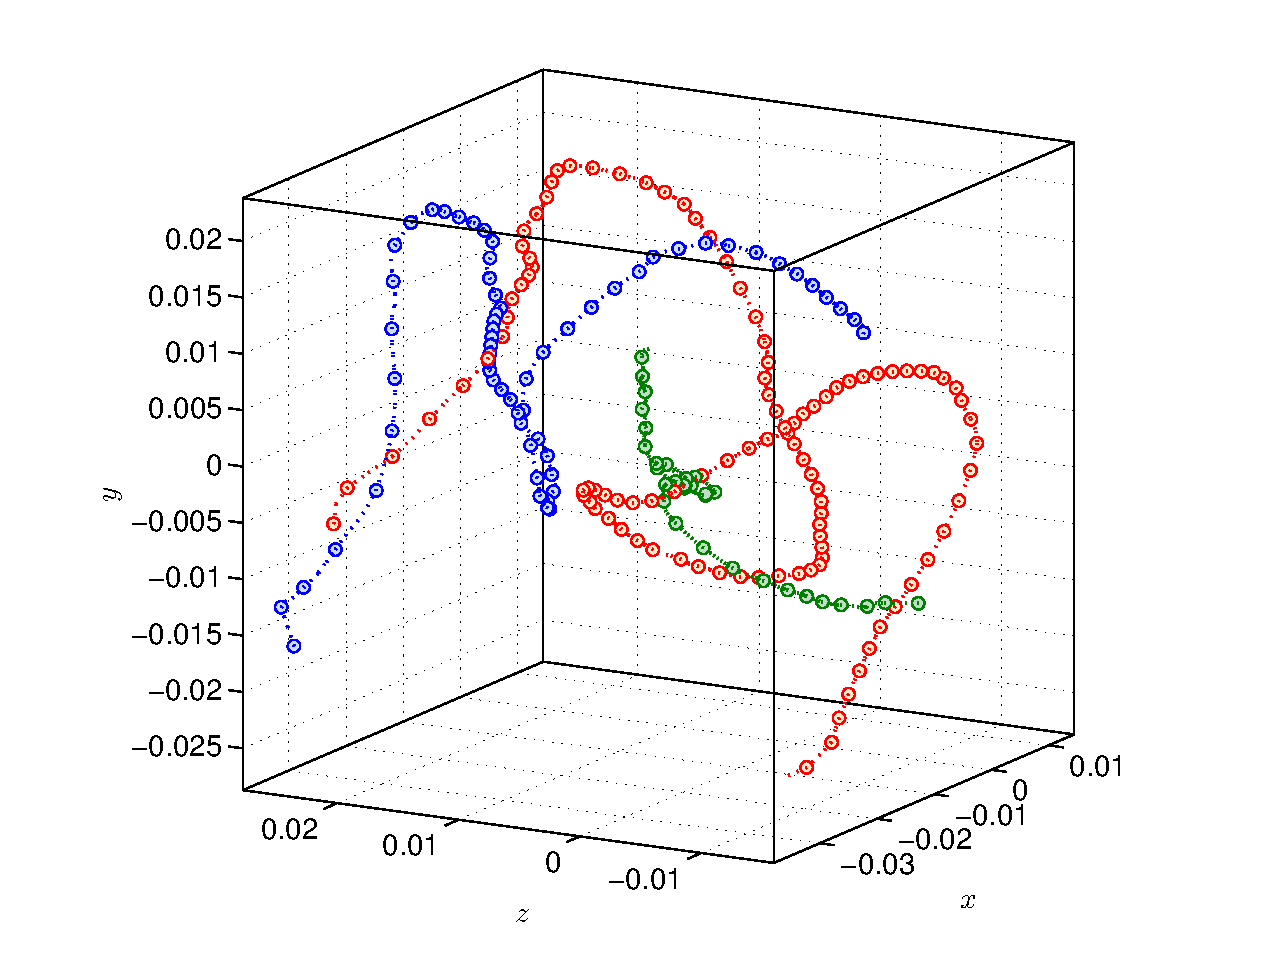
\includegraphics[width=0.8\textwidth]{few_long_trajectories}
\par\end{centering}

\caption{Some caption for the figure. Don't forget adding label to the figure
and later using the cross-reference to it. \label{fig:Some-caption-for}}


\end{figure}



\section{Tables}

\begin{table}
\begin{tabular}{|c|c|c|}
\hline 
row 1 & cell 1 & cell 2\tabularnewline
\hline 
\hline 
row 2 & cell 1 & cell 2\tabularnewline
\hline 
\end{tabular}

\caption{Table float first using Insert - > Float -> Table}


\end{table}


\begin{comment}
Use: Insert Note -> Insert List/TOC -> Bibtex Bibliography
\end{comment}




\begin{comment}
Then in the text you can use Insert citation (use the icon for the
quick use)
\end{comment}



\section{Citations}

The file references.bib in this folder is an example of how to organize
the bibliography database. It is very simple to add a reference/citation
to one of the items in the bibliography list, e.g. see the best source
of information regarding the OpenPTV origins: \citet{Dracos1996}.
Simply use: Insert -> Citation and choose from the list on the left.
Add it to the list on the right and you'll be able to choose the format
of author-year or author-number or just number to the references.
At the same time, at the end of the document you'll find References
chapter with all the cited references automatically chosen and included. 
